\subsection*{Compiler Compilers}

While you have handcrafted your (first) lexical scanner in the last exercise, 
you will explore \emph{scanner generators}, 
as part of a so-called \emph{compiler compiler}, in this %{optional} 
exercise. 
For a given grammar, these compiler compilers create the building blocks of a compiler, particularly the scanning parsing framework.
In this exercise, we will focus on the scanner, whereas its interplay with the parse will be treated later in the course.

Specifically, we will work with \textbf{JavaCC}\footnote{\url{https://javacc.github.io/javacc/}}, which represents such a compiler compiler. 
The figure below depicts the components created by JavaCC; a scanner and a parser. It illustrates their usage on an example of analyzing the String \texttt{"Total = price + tax;"}
\begin{figure}[h]
	\centering
	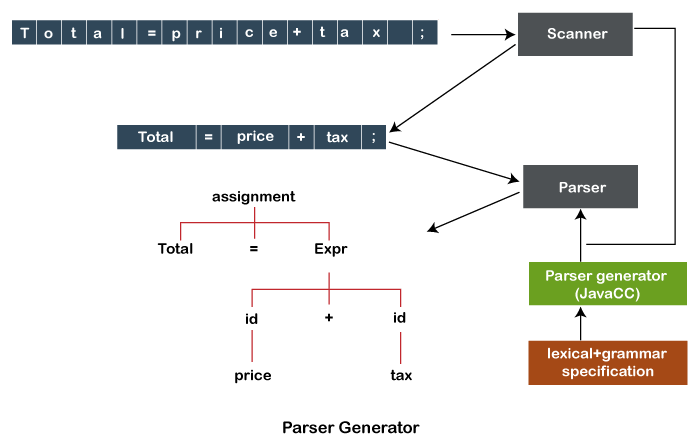
\includegraphics[width=0.7\linewidth]{figures/javacc2.png}
	\caption{JavaCC architecture taken from {\footnotesize \url{https://www.javatpoint.com/javacc}}}
\end{figure}

We will use JavaCC to automatically create a scanner and a parser and explore the created scanner in this exercise.


\begin{questions}

\titledquestion{JavaCC Basics}

To become familiar with JavaCC, you may have a look at the following documentation and tutorials: 
The list compiles a selection of tutorials to start with JavaCC:
\begin{enumerate}[
	start=1, 
	label={\upshape\bfseries D\arabic*},
	wide = 0.4cm, 
	leftmargin = 3em
	]
	\item JavaPoint: \url{https://www.javatpoint.com/javacc}
	\item Tutorial Book: 
	\url{https://www.engr.mun.ca/~theo/JavaCC-Tutorial/javacc-tutorial.pdf}
	\item Lexical Scanner Documentation: 
	\url{https://javacc.github.io/javacc/tutorials/token-manager.html}
	\item Explanation and Demo:\\ \url{https://www.infoworld.com/article/2076269/build-your-own-languages-with-javacc.html}
\end{enumerate}

\begin{parts}
	
\part Install JavaCC as described in D1 or the JavaCC main installation page at github.
	
\part Proceed with the following steps which are inspired by D4
\begin{enumerate}
	\setcounter{enumi}{0}
	\item Define a demo grammar in JavaCC, e.g., in a file \texttt{Arithmetic.jj}
	\item Execute JavaCC \texttt{javacc Arithmetic.jj}\\
	This step always generates the following Java classes:
		\begin{itemize}
			\item \textbf{\texttt{SimpleCharStream.java}}:
			 which represents the stream of input characters
			\item \textbf{\texttt{Token.java}}: which represents a single input token. 
			\item \texttt{TokenMgrError.java} which enumerates and reports the errors (if any) thrown by the token manager.
			\item \texttt{ParseException.java}
			which may report that the input does not conform to the defined grammar.
		\end{itemize}
	Plus additional classes to scan and parse the defined grammar. Let us assume the grammar is called ``Arithmetic'', 
	it will create the following additional classes:
	\begin{itemize}
		\item \texttt{Arithmetic.java}: which represents the entire parsing framework
		\item \texttt{ArithmeticTokenManager.java} which represents the lexical analyzer that breaks an input stream into tokens and assigns the type
		\item \texttt{ArithmeticConstants.java} which associates tokens with symbolic names (and numbers)
	\end{itemize}

\end{enumerate}
	You can see how tokens defined in the grammar are converted into tokens recognized by the respective \texttt{TokenManager} and represented as respective \textbf{Constants}.
\end{parts}


\medspace
\titledquestion{Create the parsing framework for SPL'}

	
Given the basic knowledge of how to use the generator of JavaCC, 
 now we employ it to generate and use \textbf{the lexical scanner} for SPL'.

\begin{parts}	
\part Define the parts of the SPL' grammar which are necessary to create the scanner in the syntax used by JavaCC. 
In the file \texttt{spl\_prime.jj}
	\begin{itemize}[noitemsep]
		\item define \texttt{SKIP} characters, particularly this shall be used to escape comments.
		\item define \texttt{TOKEN}s which recognize all the tokens defined in the previous exercise. 
		\item for this moment, you can leave the parser class empty: 
		\begin{verbatim}
			PARSER\_BEGIN(SPLPrime)
			    public class SPLPrime{ }
			PARSER\_END(SPLPrime)
		\end{verbatim}
	
	\end{itemize}
% in a file \texttt{spl\_prime.jj} nur lexikalisher anteil bislang

\part Run JavaCC to generate the lexical scanner and parser.

	The generator creates the respective classes, as mentioned in the previous task, for scanning (and parsing) \texttt{SPL'} files.

\part Test the lexical scanner by employing the input file from the previous task. 
To do so:
\begin{itemize}
	\item initiate the SPLPrime class with the byte stream
	\item employ the static method \texttt{getNextToken()} of the main (parser) class (\texttt{SPLPrime})
\end{itemize}

\end{parts}

\medspace

\textbf{Tips for defining the grammar:}
\begin{itemize}
	\item consider the \emph{order} of specifying tokens
	\item to continue skipping characters you can declare \texttt{`$\sim$'} and mention the ending character. \\
	For instance, ~ 
	\texttt{ SKIP :\{"a"}   $\sim$ \texttt{"z" \}} ~
	skips all characters between the first appearance of "a" and the first appearance of "z" 
\end{itemize}	
	
\end{questions}
